\documentclass[accentcolor=tud8b,colorbacktitle,inverttitle,landscape,german,presentation,t]{tudbeamer}
\usepackage[utf8]{inputenc}
\usepackage[ngerman]{babel}
\usepackage{graphicx}
\usepackage{listings}
\usepackage{tabto}
\usepackage{tikz}
\usetikzlibrary{shapes}

\begin{document}
% k(!)leinschrebung am Punktanfang; GIT/git -> Git
\title[Git-Workshop]{How to git gud!\\Einführung in die Quellcodeverwaltung mit Git}
\subtitle{Janika Krull\\Tim Pollandt\\\small{basierend auf Material von Steffen Klee und Jannik Vieten}}

\author[J. Krull, T. Pollandt]{Janika Krull, Tim Pollandt}
\institute[Fachschaft Informatik, TU Darmstadt]{Fachschaft Informatik, TU Darmstadt}

\logo[1]{
\includegraphics{bildmarke_ohne_rand}}
% \logo{\color{tudtextaccent}\large IFP}

\lstset{language=sh,basicstyle=\ttfamily\small, keywordstyle=\color{blue!80!black}, identifierstyle=, commentstyle=\color{green!50!black}, stringstyle=\ttfamily,
 tabsize=4, breaklines=true, numbers=left, numberstyle=\small, frame=single, backgroundcolor=\color{blue!3}}

\date{\today}

\begin{titleframe}
	\makebox(1,28)[]{}
	\begin{figure}[ht]
	\centering
  	
\includegraphics[height=60px]{git_logo}
	%\caption{gestaucht}
	%\label{fig2}
	\end{figure}
\end{titleframe}


\section{Einführung}
	\subsection{Warum Git?}
		\begin{frame}
			\frametitle{Warum Quellcodeverwaltung?}
				\begin{tikzpicture}[remember picture, note/.style={ellipse callout, fill=red!50}]
    				\node [note=blue!50, text width=3.5cm, opacity=0.90, overlay, callout absolute pointer={(-0.3,-2)}] at (3,-0.2) {Ich habe euch meinen Code doch per E-Mail geschickt.};
  				\end{tikzpicture}
  				\begin{tikzpicture}[remember picture, note/.style={ellipse callout, fill=green!50}]
    				\node [note=blue!50, text width=4cm, opacity=0.90, overlay, callout absolute pointer={(12.3,-2)}] at (8.5,-1.5) {Nein, die andere E-Mail!};
  				\end{tikzpicture}
		\end{frame}

		\begin{frame}
			\frametitle{Warum Quellcodeverwaltung?}
				\begin{tikzpicture}[remember picture, note/.style={ellipse callout, fill=red!50}]
    				\node [note=blue!50, text width=3.5cm, opacity=0.90, overlay, callout absolute pointer={(-0.3,-2)}] at (3,-0.2) {Ich habe euch meinen Code doch per E-Mail geschickt.};
  				\end{tikzpicture}
  				\begin{tikzpicture}[remember picture, note/.style={ellipse callout, fill=green!50}]
    				\node [note=blue!50, text width=4cm, opacity=0.90, overlay, callout absolute pointer={(12.3,-2)}] at (8.5,-1.5) {Nein, die andere E-Mail!};
  				\end{tikzpicture}
  				
  				\begin{tikzpicture}[remember picture, note/.style={ellipse callout, fill=red!50}]
    				\node [note=blue!50, text width=3.5cm, opacity=0.90, overlay, callout absolute pointer={(-0.3,-2)}] at (3,-3) {Jaja, ich lege es gleich in die Cloud.};
  				\end{tikzpicture}
  				\begin{tikzpicture}[remember picture, note/.style={ellipse callout, fill=green!50}]
    				\node [note=blue!50, text width=3.5cm, opacity=0.90, overlay, callout absolute pointer={(12.3,-2)}] at (8.5,-4) {Ach, ihr habt die Datei auch geändert???};
  				\end{tikzpicture}
		\end{frame}
		
		\begin{frame}
			    \frametitle{Warum Quellcodeverwaltung?}
			    	\begin{tikzpicture}[remember picture, note/.style={ellipse callout, fill=yellow!50}]
    				\node [note=blue!50, text width=4.3cm, opacity=0.90, overlay, callout absolute pointer={(3,-4)}] at (6,-2) {Das ging doch mal!\\Wer hat das denn geändert?\\Am liebsten hätte ich wieder den Stand von gestern.};
  				\end{tikzpicture}
		\end{frame}
		
		\begin{frame}
			\frametitle{Darum Quellcodeverwaltung!}
				\begin{itemize}
					\item jederzeit erreichbares \textbf{zentrales Quellcodeverzeichnis}
					\item \textbf{offline} speicher- und verwaltbar
					\item keine Probleme bei \textbf{gleichzeitiger Bearbeitung} \textit{verschiedener} Dateien
					\item \textbf{Konfliktlösung} bei gleichzeitiger Bearbeitung \textit{gleicher} Dateien möglich
					\item \textbf{Wiederherstellung} alter Versionen und \textit{Revidieren} einzelner Änderungen möglich
					\item \textbf{Übersicht} über Änderungen der Anderen
					\item große Änderungen können getrennt entwickelt und auf einmal in das Hauptverzeichnis übernommen werden
					\item uvm.
				\end{itemize}
		\end{frame}
		\begin{frame}
			\frametitle{Warum Git?}
				\begin{itemize}
					\item Git ist eine der wichtigsten Lösungen zur Quellcodeverwaltung
					\item von Linus Torvalds 2005 initiiert
					\item das im \textit{Open Source}-Bereich oft genutzte \textbf{GitHub} basiert auf Git
					\item Git ist in \underline{https://scm.informatik.tu-darmstadt.de} verfügbar
					\item Git ist auf eigenen Servern leicht zu hosten
					\item[\checkmark] Just do Git!
					\item Alternativen sind zum Beispiel \textbf{Mercurial} und \textbf{SVN}
				\end{itemize}
		\end{frame}
		
\section{Funktionsweise}
	 \subsection{Normalfall}
		\begin{frame}
			\frametitle{Funktionsweise}
				\begin{tikzpicture}
					\definecolor{lightblue}{HTML}{7F7FFF}
					\definecolor{darkgreen}{HTML}{00A700}
					\draw[very thick] (0,0) -- (0, 5.9);
					\draw[very thick,blue,fill=lightblue] (0,0.5) -- (0.2,0.7) -- (0,0.9) -- (-0.2,0.7) -- (0,0.5);
					\draw[very thick,blue,fill=lightblue] (0,2.03) -- (0.2,2.23) -- (0,2.43) -- (-0.2,2.23) -- (0,2.03);
					\draw[very thick,blue,fill=lightblue] (0,3.57) -- (0.2,3.77) -- (0,3.97) -- (-0.2,3.77) -- (0,3.57);
					\draw[very thick,blue,fill=lightblue] (0,5) -- (0.2,5.2) -- (0,5.4) -- (-0.2,5.2) -- (0,5);
					
					\node[anchor=west] at (-2,0.69) {\texttt{54cdb2c}};
					\node[anchor=west] at (-2,2.22) {\texttt{f39a8c8}};
					\node[anchor=west] at (-2,3.76) {\texttt{7854994}};
					\node[anchor=west] at (-2,5.19) {\texttt{1f42b40}};
					
					\node[anchor=west] at (1,0.69) {\textbf{Revert: implemented add}};
					\node[anchor=west] at (1,0.29) {Wir müssen das nicht};
					\node[anchor=west] at (1,0) {manuell schreiben!};
					\node[anchor=west] at (1,2.22) {\textbf{implemented sub}};
					\node[anchor=west] at (1,3.76) {\textbf{implemented add}};
					\node[anchor=west] at (1,3.36) {solved task 1};
					\node[anchor=west] at (1,5.19) {\textbf{initial commit}};
					
					\node[draw,anchor=west] at (6,0.7) {\small\texttt{\begin{tabular}{rl} &(define (add a b) \\ \textcolor{darkgreen}{+}&\textcolor{darkgreen}{;;TODO implement} \\ \textcolor{red}{-}&\hspace*{0.5cm}\textcolor{red}{(+ a b)}\\&) \end{tabular}}};
					\node[draw,anchor=west] at (4,2.35) {\small\texttt{\begin{tabular}{rl} &(define (sub a b) \\ \textcolor{red}{-}&\textcolor{red}{;;TODO implement} \\ \textcolor{darkgreen}{+}&\hspace*{0.5cm}\textcolor{darkgreen}{(- a b)}\\&) \end{tabular}}};
					\node[draw,anchor=west] at (6,4) {\small\texttt{\begin{tabular}{rl} &(define (add a b) \\ \textcolor{red}{-}&\textcolor{red}{;;TODO implement} \\ \textcolor{darkgreen}{+}&\hspace*{0.5cm}\textcolor{darkgreen}{(+ a b)}\\&) \end{tabular}}};
					\node[draw,anchor=west] at (3.5,5.15) {\tiny\texttt{\begin{tabular}{rl} \textcolor{darkgreen}{+}&\textcolor{darkgreen}{(define (add a b)} \\ \textcolor{darkgreen}{+}&\textcolor{darkgreen}{;;TODO implement}\\\textcolor{darkgreen}{+}&\textcolor{darkgreen}{)}\\\textcolor{darkgreen}{+}&\textcolor{darkgreen}{(define (sub a b)} \\ \textcolor{darkgreen}{+}&\textcolor{darkgreen}{;;TODO implement}\\\textcolor{darkgreen}{+}&\textcolor{darkgreen}{)} \end{tabular}}};
				\end{tikzpicture}
		\end{frame}
		\begin{frame}
			\frametitle{Schritte in Git (Normalfall)}
				\begin{tabular}{lcl}
					\texttt{git pull} & Änderungen herunter-/hochladen & \texttt{git push}\\
					\texttt{git checkout} & Änderungen in Entwicklungsbranch einfügen & \texttt{git commit}\\
					\texttt{vi \textit{<Datei>}} \tiny{[z. B.]} & Dateien ändern/hinzufügen &  \texttt{git add}\\
				\end{tabular}
				\put(-349,-15){
					\definecolor{darkgreen}{HTML}{00A700}
					\begin{tikzpicture}
						\draw[->,very thick,red] (0,1.2) -- (0, 0);
						\draw[->,very thick,darkgreen] (12.1,0) -- (12.1, 1.2);
					\end{tikzpicture}
				}
				
					\makebox(1,136)[]{}				
					\centering
					\begin{tikzpicture}
						\definecolor{darkgreen}{HTML}{00A700}
						\node [cloud,fill=blue!30,draw,cloud puffs=9,cloud puff arc=150,aspect=2,inner ysep=0.8em] at (0,3.5) {Server};
						\node [cylinder,cylinder uses custom fill,cylinder body fill=yellow!50,cylinder end fill=yellow!30,shape border rotate=90,aspect=0.25,draw] at (0,0.3) {lokales Verzeichnis};
						\draw (-5,0) -- (-5,1.2) -- (-4.3,1.2) -- (-4.3,0.8) -- (-4,0.8) -- (-4,0) -- cycle;
						\draw (-4.3,1.2) -- (-4,0.8);
						\foreach \y in {0.2,0.4,0.6}{
     						\draw (-4.8,\y) -- (-4.2,\y);
							\draw (-4.8,0.8) -- (-4.4,0.8);
							\draw (-4.8,1) -- (-4.4,1);
						}
						\node at (-8,0.8) {
\includegraphics[width=1.5cm]{pingu-pc}};
						
						\draw[<-,very thick,red] (-7,0.7) -- (-5.2,0.7);
						\draw[->,very thick,darkgreen] (-7,0.4) -- (-5.2,0.4);
						\node[anchor=west] at (-6.95,0.95) {\textit{bearbeiten}};
						\node[anchor=west] at (-6.95,0.15) {\texttt{git add}};
						
						\draw[<-,very thick,red] (-3.8,0.7) -- (-1.75,0.7);
						\draw[->,very thick,darkgreen] (-3.8,0.4) -- (-1.75,0.4);
						\node[anchor=west] at (-3.85,0.95) {\small\texttt{git checkout}};
						\node[anchor=west] at (-3.85,0.15) {\texttt{git commit}};
						
						\draw[<-,very thick,red] (-0.15,0.9) -- (-0.15,2.6);
						\draw[->,very thick,darkgreen] (0.15,0.9) -- (0.15,2.6);
						\node[anchor=east] at (-0.2,2) {\texttt{git pull}};
						\node[anchor=west] at (0.2,2) {\texttt{git push}};
					\end{tikzpicture}
		\end{frame}
	\subsection{Abweichungen vom Normalfall}
		\subsubsection{Gleichzeitig bearbeitet}
			\begin{frame}
			\frametitle{Gleichzeitiges Bearbeiten}
				Wir nehmen den folgenden Fall an:
				\begin{itemize}
					\item \textbf{Alice} lädt Änderungen auf Computer \textbf{A} herunter (\textit{git pull}).
					\item \textbf{Bob} lädt Änderungen auf Computer \textbf{B} herunter (\textit{git pull}).
					\item \textbf{Alice} und \textbf{Bob} bearbeiten verschiedene Dateien und committen diese.
					\item \textbf{Alice} lädt ihre Änderungen hoch (\textit{git push}).
					\item \textbf{Bob } versucht seine Änderungen hochzuladen (\textit{git push}).
					\item [\textbf{error}] (beide Verzeichnisse wurden bearbeitet)
				\end{itemize}
				
				Da Bobs Änderung noch auf der Version vor Alice' Änderung basiert,\\
				kann sie nicht einfach übertragen werden (um nichts zu überschreiben).\\
				\begin{itemize}
					\item \textbf{Lösung:} Versionen lokal zusammenführen
				\end{itemize}
			\end{frame}
			
			\begin{frame}
				\frametitle{Gleichzeitiges Bearbeiten}
					\centering
					\begin{tikzpicture}
					\definecolor{lightblue}{HTML}{7F7FFF}
					\definecolor{darkgreen}{HTML}{00A700}
					\draw[very thick] (0,2.35) -- (0, 5.9);
					\draw[very thick] (0,5.2) -- (2.15, 3.05);
					\draw[very thick] (2.15,3.05) -- (2.15, 2.35);
					\draw[very thick,blue,fill=lightblue] (0,2.85) -- (0.2,3.05) -- (0,3.25) -- (-0.2,3.05) -- (0,2.85);
					\draw[very thick,blue,fill=lightblue] (0,5) -- (0.2,5.2) -- (0,5.4) -- (-0.2,5.2) -- (0,5);
					\draw[very thick,blue,fill=lightblue] (2.15,2.85) -- (2.35,3.05) -- (2.15,3.25) -- (1.95,3.05) -- (2.15,2.85);
					
					\node[draw,anchor=east] at (-0.5,3) {\small\texttt{\begin{tabular}{rl} &(define (sub a b) \\ \textcolor{red}{-}&\textcolor{red}{;;TODO implement} \\ \textcolor{darkgreen}{+}&\hspace*{0.5cm}\textcolor{darkgreen}{(- a b)}\\&) \end{tabular}}};
					\node[draw,anchor=west] at (2.65,3) {\small\texttt{\begin{tabular}{rl} &(define (add a b) \\ \textcolor{red}{-}&\textcolor{red}{;;TODO implement} \\ \textcolor{darkgreen}{+}&\hspace*{0.5cm}\textcolor{darkgreen}{(+ a b)}\\&) \end{tabular}}};
					\node[draw,anchor=east] at (-0.5,5.2) {\tiny\texttt{\begin{tabular}{rl} \textcolor{darkgreen}{+}&\textcolor{darkgreen}{(define (add a b)} \\ \textcolor{darkgreen}{+}&\textcolor{darkgreen}{;;TODO implement}\\\textcolor{darkgreen}{+}&\textcolor{darkgreen}{)}\\\textcolor{darkgreen}{+}&\textcolor{darkgreen}{(define (sub a b)} \\ \textcolor{darkgreen}{+}&\textcolor{darkgreen}{;;TODO implement}\\\textcolor{darkgreen}{+}&\textcolor{darkgreen}{)} \end{tabular}}};
				\end{tikzpicture}
			\end{frame}
			
			\begin{frame}
				\frametitle{Gleichzeitiges Bearbeiten}
					\centering
					\begin{tikzpicture}
					\definecolor{lightblue}{HTML}{7F7FFF}
					\definecolor{darkgreen}{HTML}{C07700}
					\draw[very thick] (0,2.35) -- (0, 5.9);
					\draw[very thick] (0,5.2) -- (2.15, 3.05);
					\draw[very thick] (2.15,3.05) -- (2.15, 2.35);
					\draw[very thick,blue,fill=lightblue] (0,2.85) -- (0.2,3.05) -- (0,3.25) -- (-0.2,3.05) -- (0,2.85);
					\draw[very thick,blue,fill=lightblue] (0,5) -- (0.2,5.2) -- (0,5.4) -- (-0.2,5.2) -- (0,5);
					\draw[very thick,blue,fill=lightblue] (2.15,2.85) -- (2.35,3.05) -- (2.15,3.25) -- (1.95,3.05) -- (2.15,2.85);
					
					\node[draw,anchor=west] at (2.65,4) {\texttt{\begin{tabular}{l} (define (add a b) \\ \textcolor{darkgreen}{\hspace*{0.5cm}(+ a b)}\\)\\(define (sub a b) \\ ;;TODO implement \\) \end{tabular}}};
					\node[draw,anchor=east] at (-0.5,3) {\texttt{\begin{tabular}{l} (define (add a b) \\ ;;TODO implement\\)\\(define (sub a b) \\ \textcolor{darkgreen}{\hspace*{0.5cm}(- a b)}\\) \end{tabular}}};
					\node[draw,anchor=east] at (-0.5,5.2) {\tiny\texttt{\begin{tabular}{l} \textcolor{darkgreen}{(define (add a b)} \\ \textcolor{darkgreen}{;;TODO implement}\\\textcolor{darkgreen}{)}\\\textcolor{darkgreen}{(define (sub a b))} \\ \textcolor{darkgreen}{;;TODO implement}\\\textcolor{darkgreen}{)} \end{tabular}}};
				\end{tikzpicture}
			\end{frame}
			
			\begin{frame}
				\frametitle{Gleichzeitiges Bearbeiten}
					\centering
					\begin{tikzpicture}
					\definecolor{lightblue}{HTML}{7F7FFF}
					\definecolor{darkgreen}{HTML}{C07700}
					\draw[very thick] (0,0) -- (0, 5.9);
					\draw[very thick] (0,5.2) -- (2.15, 3.05);
					\draw[very thick] (0,0.7) -- (2.15, 3.05);
					\draw[very thick,blue,fill=lightblue] (0,0.5) -- (0.2,0.7) -- (0,0.9) -- (-0.2,0.7) -- (0,0.5);
					\draw[very thick,blue,fill=lightblue] (0,2.85) -- (0.2,3.05) -- (0,3.25) -- (-0.2,3.05) -- (0,2.85);
					\draw[very thick,blue,fill=lightblue] (0,5) -- (0.2,5.2) -- (0,5.4) -- (-0.2,5.2) -- (0,5);
					\draw[very thick,blue,fill=lightblue] (2.15,2.85) -- (2.35,3.05) -- (2.15,3.25) -- (1.95,3.05) -- (2.15,2.85);
					
					\node[draw,anchor=west] at (2.65,4) {\texttt{\begin{tabular}{l} (define (add a b) \\ \textcolor{darkgreen}{\hspace*{0.5cm}(+ a b)}\\)\\(define (sub a b) \\ ;;TODO implement \\) \end{tabular}}};
					\node[draw,anchor=east] at (-0.5,3) {\texttt{\begin{tabular}{l} (define (add a b) \\ ;;TODO implement\\)\\(define (sub a b) \\ \textcolor{darkgreen}{\hspace*{0.5cm}(- a b)}\\) \end{tabular}}};
					\node[draw,anchor=east] at (-0.5,5.2) {\tiny\texttt{\begin{tabular}{l} \textcolor{darkgreen}{(define (add a b)} \\ \textcolor{darkgreen}{;;TODO implement}\\\textcolor{darkgreen}{)}\\\textcolor{darkgreen}{(define (sub a b))} \\ \textcolor{darkgreen}{;;TODO implement}\\\textcolor{darkgreen}{)} \end{tabular}}};
					\node[draw,anchor=west] at (1.8,1) {\texttt{\begin{tabular}{l} (define (add a b) \\ \textcolor{darkgreen}{\hspace*{0.5cm}(+ a b)}\\)\\(define (sub a b) \\ \textcolor{darkgreen}{\hspace*{0.5cm}(- a b)}\\) \end{tabular}}};
				\end{tikzpicture}
			\end{frame}
			
			\begin{frame}
				\frametitle{Versionen zusammenführen (\textit{merge})}
					Reihenfolge ist wichtig!\\ Wenn das Remote-Repository zwischendurch geändert wurde:
					\begin{enumerate}
						\item \texttt{git pull}
						\item \texttt{git push}
					\end{enumerate}
			\end{frame}
			
		\subsubsection{Merge-Konflikte}
			\begin{frame}
				\frametitle{Merge-Konflikt}
					\begin{itemize}
						\item bei Änderungen in der gleichen Zeile der gleichen Datei kann Git die Versionen nicht automatisch zusammenführen
						\item[$\rightarrow$] Merge-Konflikt
					\end{itemize}
			\end{frame}
			
			\begin{frame}
				\frametitle{Merge-Konflikt}
					\centering
					\begin{tikzpicture}
					\definecolor{lightblue}{HTML}{7F7FFF}
					\definecolor{darkgreen}{HTML}{C07700}
					\draw[very thick] (0,0) -- (0, 5.9);
					\draw[very thick] (0,5.2) -- (2.15, 3.05);
					\draw[very thick, dashed] (0,0.7) -- (1, 1.7);
					\draw[very thick] (1.15,2.05) -- (2.15, 3.05);
					\draw[very thick,red,fill=lightblue] (0,0.5) -- (0.2,0.7) -- (0,0.9) -- (-0.2,0.7) -- (0,0.5);
					\draw[very thick,blue,fill=lightblue] (0,2.85) -- (0.2,3.05) -- (0,3.25) -- (-0.2,3.05) -- (0,2.85);
					\draw[very thick,blue,fill=lightblue] (0,5) -- (0.2,5.2) -- (0,5.4) -- (-0.2,5.2) -- (0,5);
					\draw[very thick,blue,fill=lightblue] (2.15,2.85) -- (2.35,3.05) -- (2.15,3.25) -- (1.95,3.05) -- (2.15,2.85);
					\draw[->,>=stealth,very thick, red] (1.25,2.5)--++(-0.3,-0.7)--++(0.4,0.25)--++(-0.3,-0.7);
					
					\node[draw,anchor=west] at (2.65,3) {\texttt{\begin{tabular}{l} (define (add a b) \\ \textcolor{darkgreen}{\hspace*{0.5cm}(+ a b)}\\)\\(define (sub a b) \\ \textcolor{darkgreen}{\hspace*{0.5cm}(+ a (* -1 b))} \\) \end{tabular}}};
					\node[draw,anchor=east] at (-0.5,3) {\texttt{\begin{tabular}{l} (define (add a b) \\ ;;TODO implement\\)\\(define (sub a b) \\ \textcolor{darkgreen}{\hspace*{0.5cm}(- a b)}\\) \end{tabular}}};
					\node[draw,anchor=east] at (-0.5,5.2) {\tiny\texttt{\begin{tabular}{l} \textcolor{darkgreen}{(define (add a b)} \\ \textcolor{darkgreen}{;;TODO implement}\\\textcolor{darkgreen}{)}\\\textcolor{darkgreen}{(define (sub a b))} \\ \textcolor{darkgreen}{;;TODO implement}\\\textcolor{darkgreen}{)} \end{tabular}}};
					\node[red] at (2.2,0.8) {Git happens!};
				\end{tikzpicture}
			\end{frame}
			
			\begin{frame}
				\frametitle{Merge-Konflikt}
					\begin{itemize}
						\item bei Änderungen in der gleichen Zeile der gleichen Datei kann Git die Versionen nicht automatisch zusammenführen
						\item[$\rightarrow$] Merge-Konflikt
						\begin{itemize}
							\item wieder erst \textit{pullen}
							\item Merge-Konflikt manuell in Datei beheben:\\
							\lstinputlisting{merge_conflict.rkt}
							\item \textit{committen} und Commit-Name \textbf{Merge branch 'master' of  ...} ändern
							\item \textit{pushen}
						\end{itemize}
					\end{itemize}
			\end{frame}
			
		\subsubsection{Große Änderungen}
			\begin{frame}
				\frametitle{Große Änderungen auslagern}
					\begin{itemize}
						\item Branches
						\begin{itemize}
							\item[>] separate Entwicklung großer Änderungen
							\item[>] Quellcode anderer Branches ist jederzeit nutz- und änderbar
						\end{itemize}
						\item Pull Requests
						\begin{itemize}
							\item[>] Überprüfung von Änderungen durch Berechtigte
						\end{itemize}
						\item Abspaltungen (\textit{fork/clone})
						\begin{itemize}
							\item[>] Entwicklung eines auf einem anderen Projekt basierenden Codes
							\item[>] Änderungen des Originalprojekts können leicht übernommen werden
						\end{itemize}
					\end{itemize}
					\centering
					\begin{tikzpicture}
					\definecolor{lightblue}{HTML}{7F7FFF}
					\draw[very thick] (0,0) -- (10.6,0);
					\draw[very thick,purple] (0.7,0) -- (3.05,2.15);
					\draw[very thick,purple] (5.2,0) -- (3.05,2.15);
					\draw[very thick,orange] (3.05,0) -- (5.2,2.15);
					\draw[very thick,green] (5.2,2.15) -- (7.55,1.07);
					\draw[very thick,orange] (5.2,2.15) -- (10.6,2.15);
					\draw[very thick,green] (7.55,1.07) -- (10.6,1.07);
					\draw[very thick,blue,fill=lightblue] (0.5,0) -- (0.7,0.2) -- (0.9,0) -- (0.7,-0.2) -- (0.5,0);
					\draw[very thick,blue,fill=lightblue] (2.85,0) -- (3.05,0.2) -- (3.25,0) -- (3.05,-0.2) -- (2.85,0);
					\draw[very thick,blue,fill=lightblue] (5,0) -- (5.2,0.2) -- (5.4,0) -- (5.2,-0.2) -- (5,0);
					\draw[very thick,blue,fill=lightblue] (5,2.15) -- (5.2,2.35) -- (5.4,2.15) -- (5.2,1.95) -- (5,2.15);
					\draw[very thick,blue,fill=lightblue] (7.35,0) -- (7.55,0.2) -- (7.75,0) -- (7.55,-0.2) -- (7.35,0);
					\draw[very thick,blue,fill=lightblue] (7.35,1.07) -- (7.55,1.27) -- (7.75,1.07) -- (7.55,0.87) -- (7.35,1.07);
					\draw[very thick,blue,fill=lightblue] (9.7,1.07) -- (9.9,1.27) -- (10.1,1.07) -- (9.9,0.87) -- (9.7,1.07);
					\draw[very thick,blue,fill=lightblue] (9.7,0) -- (9.9,0.2) -- (10.1,0) -- (9.9,-0.2) -- (9.7,0);
					\draw[very thick,blue,fill=lightblue] (2.85,2.15) -- (3.05,2.35) -- (3.25,2.15) -- (3.05,1.95) -- (2.85,2.15);
					\draw[very thick,blue,fill=lightblue] (8.53,2.15) -- (8.73,2.35) -- (8.93,2.15) -- (8.73,1.95) -- (8.53,2.15);
				\end{tikzpicture}
			\end{frame}
		\subsubsection{Rebase}
			\begin{frame}
				\frametitle{Änderungen zusammenfassen}
					\begin{itemize}
						\item Zu viele Commits für eine Änderung sind oft unerwünscht
						\item man kann mehrere Commits zu einem zusammenfassen:
						\item \texttt{git rebase -i HEAD$\sim$3} listet die letzten 3 Commits auf
						\item nun kann man beim zu entfernenden Commit \texttt{pick} in \texttt{squash} ändern
						\item dieser wird in den vorherigen eingefügt
						\item der Name sollte wieder sinnvoll vergeben werden
						\item nun kann der Vorgang mit \texttt{git rebase -{-}continue} abgeschlossen werden 
					\end{itemize}
			\end{frame}

\section{Sinnvolles Verhalten}

			\begin{frame}
				\frametitle{\texttt{.gitignore}-Datei}
				Mithilfe von \texttt{.gitignore}-Dateien, kann man festlegen, welche Dateien (nicht) mit git synchronisiert werden.
				\lstinputlisting{example.gitignore}
			\end{frame}
			
			\begin{frame}
				\frametitle{How to git gud!}
					\begin{itemize}
						\item sinnvolle Commit-Mitteilungen schreiben
						\item Binärdateien u. ä. in \texttt{.gitignore}-Datei aufnehmen
						\item spätestens vor \texttt{push} alles Tests laufen lassen
						\item semantisch zusammenhängende Änderungen in einen Commit packen
					\end{itemize}
			\end{frame}
			
			\begin{frame}
				\frametitle{Es git viele weitere Befehle!}
					\begin{tabular}{ll}
						\texttt{git pull} & Änderungen herunterladen\\
						\texttt{git push} & Änderungen hochladen\\
						\texttt{git checkout} & Branch auswählen\\
						\texttt{git add <-A>} & Dateien hinzufügen\\
						\texttt{git commit <-a>} & Commit erstellen\\
						\texttt{git diff} & Versionsunterschiede anzeigen\\
						\texttt{git log <-{-}pretty=oneline>} & Versionsgeschichte anzeigen\\
						\texttt{git rebase -i HEAD$\sim$3} & Commits zusammenlegen\\&(danach \texttt{git rebase -{-}continue})\\
						\texttt{git help} & Hilfe zu Git\\
						\texttt{git \textit{<Befehl>} -{-}help} & Hilfe zu Git-Befehlen
					\end{tabular}
			\end{frame}
		
\section{Ende}			
			
			\begin{frame}
				\frametitle{Vielen Dank für eure Aufmerksamkeit!}
					\begin{figure}[]
						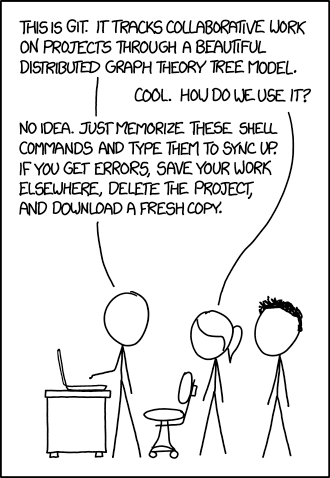
\includegraphics[height=150px]{git_comic}
						\caption{https://xkcd.com/1597/}
						\label{fig1}
					\end{figure}
			\end{frame}
			
\section{Praxis}
			\begin{frame}
				\frametitle{Praxis:\\\texttt{commit} ins Abenteuerland}
					\begin{itemize}
						\item Verbinden mit dem WLAN
						\NumTabs{7}
						\begin{itemize}
							\item SSID: \tab\textbf{Git Workshop}
							\item Passwort: \tab\textbf{ofahrt2017git}
						\end{itemize}
						\item \underline{http://workshop.lan} aufrufen
						\item Daten herunterladen und installieren/bearbeiten
					\end{itemize}
			\end{frame}			
			
			\end{document}

